\documentclass[journal,a4paper]{IEEEtran}

\usepackage{algorithm}
\usepackage{algorithmic}

\usepackage{pgfplots}
\pgfplotsset{compat=1.9}

\usepackage[british]{babel}

\begin{document}

\title{An Adaptive Prefetcher Based on Delta-Correlating Prediction Tables and Reference Prediction Tables}
\author{Olav-Emil Eiksund, Christopher Lohne, Kristian Klomsten Skordal}
\maketitle

\begin{abstract}
This article describes an algorithm for L2 prefetching that combines the use of
delta-correlating prediction tables (DCPT) and reference prediction tables in
order to get improved prefetcher accuracy under varying conditions.

Under our simulated conditions, a speedup of 7.6~\% was observed as compared to
using no prefetcher.
\end{abstract}

\section{Introduction}
\IEEEPARstart{O}{ur} prefetcher is so awesome, and this paragraph has to be two
lines long in order for the hanging first letter to look cool.

\section{Related Work or Background}
Insert related work and/or background here.

\section{Prefetcher Description}
The implemented prefetcher combines an RPT and a DCPT prefetcher and
switches between them in order to achieve the highest possible performance.
Both the DCPT and RPT implementation uses 22 bit deltas and partial matching
with an 8 bit mask to improve performance.

This is done by running both algorithms alternatively and tracking their
accuracy. At a predefined number of cache misses, an algorithm decides if the
currently running prefetcher algorithm should be switched. The switching
algorithm gives preference to the prefetcher algorithm having the highest
accuracy when deciding which algorithm to switch to, but is designed to allow
the other algorithm to run as well to accomodate changes in the running
programme environment.

The switching algorithm works by first using a random number generator to
choose a number between 0 and 100. Then, the accuracy of the algorithm with the
highest accuracy is multiplied by 100, giving the percentage accuracy of the
algorithm. This is then used to choose the algorithm to switch to; if the randomly
selected number is lower than or equal to the percentage accuracy of the highest
performing algorithm, that algorithm is selected, otherwise the other algorithm
is selected. The algorithm is illustrated in figure \ref{fig:switching}.

\begin{figure}[!h]
	\caption{Algorithm for switching between prefetchers}
	\label{fig:switching}
	\centering

	\begin{algorithmic}[1]
		\STATE $R \leftarrow \textrm{rand(0, 100)}$
		\IF{DCPT-P has higher accuracy}
			\IF{$\textrm{DCPT.accuracy} * 100 <= R$}
				\STATE $\textrm{Algorithm} \leftarrow \textrm{DCPT}$
			\ELSE
				\STATE $\textrm{Algorithm} \leftarrow \textrm{RPT}$
			\ENDIF
		\ELSIF{RPT has higher accuracy}
			\IF{$\textrm{RPT.accuracy} * 100 <= R$}
				\STATE $\textrm{Algorithm} \leftarrow \textrm{RPT}$
			\ELSE
				\STATE $\textrm{Algorithm} \leftarrow \textrm{DCPT}$
			\ENDIF
		\ENDIF
	\end{algorithmic}
\end{figure}

\section{Methodology}

In order to measure the performance of the prefetcher, the speedup compared to
using no prefetcher is measured.

The main reason for a prefetcher is to make the system faster. To qualify if a
new prefetcher implementation is good it is interesting to have a number that
tells you how much faster it is. This number can be the speedup, the speedup
gives an overview of the overall performance of the prefetcher. Other important
measurements are Coverage, Accuracy, Identified, Issued and Misses. 
Simulator

The prefetcher in this paper is tested on a M5 simulator system with a subset of
SPEC CPU2000 benchmark. The M5 simulator is a software platform that allows
simulating a complete hardware system. The simulated CPU is an Alpha 21264, which
is an out-of-order processor. The memory settings used for our simulations are shown
in table \ref{tab:simsetup}. There is no prefetching for the L1 cache. Statistics
are gathered after fast-forwarding 10000000 instructions.

\begin{table}[h]
	\caption{Simulator setup\cite{userman}}
	\label{tab:simsetup}
	\centering

	\begin{tabular}{|l|l|}
		\hline
		L1 data cache & 64~kb \\
		L1 instruction cache & 32~kb \\
		L2 cache size & 1~Mb \\
		Memory bus width & 400~MHz \\
		Memory latency & 30~ns \\
		\hline
	\end{tabular}
\end{table}

%And the subset of SPEC CPU2000 contains the following tests: swim, twolf, bzip2_source,
% apsi, bizp2_graphic, galgel, bizip2_program, art470, art110, applu, wupwise and ammp. 

The simulations were run on the Kongull computer cluster at the Norwegian University
of Science and Technology. The cluster consists of 107 nodes with two six core AMD
Opteron 2431 processors on each node\cite{kongull}.

The simulations was done on our personal computers with a modified linux version with
M5 and on a computer cluster on NTNU. To run the SPEC CPU2000 in the M5 simulator a
python script was used. The python script determines which of the test in SPEC CPU2000
to run and it prints out the results from the different tests. 

\section{Results}
The measured speedup compared to pure RPT and DCPT-P implementations are presented in
figure \ref{fig:results}. The best speedup can be observed in the ammp test, where
our speedup is almost 3 times the speedup of using a pure DCPT-P prefetcher.

\begin{figure}
	\caption{Comparison of RPT, DCPT-P and A-RPT*DCPT-P prefetchers}
	\label{fig:results}
	\centering

	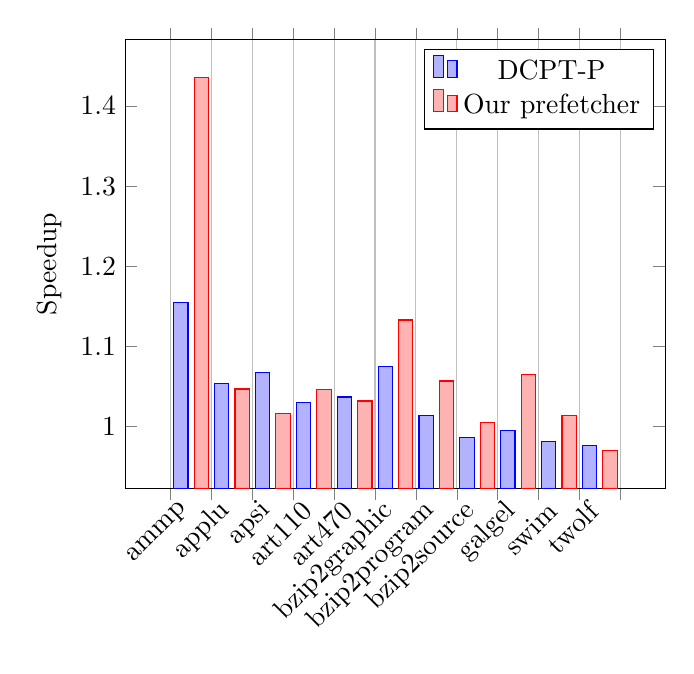
\begin{tikzpicture}
		\begin{axis}[
			ylabel=Speedup,
			ybar,
			symbolic x coords={ammp,applu,apsi,art110,art470,bzip2graphic,bzip2program,bzip2source,galgel,swim,twolf,wupwise},
			xtick=data,
			x tick label style={rotate=45,anchor=east},
			ybar interval=0.7
		]
			\addplot coordinates {(ammp,1.155) (applu,1.054) (apsi,1.068) (art110,1.030) (art470,1.037) (bzip2graphic,1.075) (bzip2program,1.014) (bzip2source,0.986) (galgel,0.995) (swim,0.982) (twolf,0.976) (wupwise,1.142)};
			\addplot coordinates {(ammp,1.436) (applu,1.047) (apsi,1.016) (art110,1.046) (art470,1.032) (bzip2graphic,1.133) (bzip2program,1.057) (bzip2source,1.005) (galgel,1.065) (swim,1.014) (twolf,0.970) (wupwise,1.240)};
			\legend{DCPT-P,Our prefetcher}
		\end{axis}
	\end{tikzpicture}
\end{figure}

\section{Discussion}
Discuss our amazing results here.

\section{Future Work}
The algorithm for switching between DCPT-P and RPT gives a better performance than
without switching. It is possible that more tweaking of when to switch and implement
a priority to DCPT-P can give a even better performance. It´s also possible that making
a more complex switching algorithm for detecting what type of data the prefetcher is
working on and give the methods that is best for this type of data can give better
performance. Another thing that is interesting too take a deeper look at is the size of
the deltas used in the DCPT-P. 

\section{Conclusion}

\begin{thebibliography}{1}
	\bibitem{kongull} NTNU High Performance Computing Group, \emph{Kongull Hardware}, \hskip 1em plus
		0.5em minus 0.4em\relax https://www.hpc.ntnu.no/display/hpc/Kongull+Hardware.
	\bibitem{userman} NTNU Computer Architecture Group, \emph{M5 Simulator System}, \hskip 1em plus
		0.5em minus 0.4em\relax NTNU, 2014.
\end{thebibliography}

\end{document}

